\documentclass{beamer}

\usepackage[T1]{fontenc}       
\usepackage[utf8]{inputenc}    % pour les accents (mettre latin1 pour windows au lieu de utf8)
\usepackage[frenchb]{babel}    % le documents est en français
\usepackage{amsmath}           % un packages mathématiques
\usepackage{xcolor}            % pour définir plus de couleurs 
\usepackage{graphicx}          % pour insérer des figures

\useoutertheme[height=0pt, width=80pt,left, hideothersubsections]{sidebar}
\usecolortheme{seahorse}
\setbeamercolor*{titlelike}{parent=structure}
\useinnertheme{circles}
\setbeamertemplate{frametitle}[default][right]
\setbeamertemplate{blocks}[rounded][shadow=true]


%Title info
\title[STM32L - Qemu]{Emulation STM32L Discovery avec Qemu}
\author{Clavelin Aurélien, Eid Timothée, Mercier Michaël}
\date{}



% Faire apparaître un sommaire avant chaque section
\AtBeginSection[]{
   \begin{frame}
   \begin{center}{\Large Plan }\end{center}
   %%% affiche en début de chaque section, les noms de sections et
   %%% noms de sous-sections de la section en cours.
   \tableofcontents[currentsection, hideallsubsections]
   \end{frame} 
}
		





% Début de la présentation
% Contenu
\begin{document}
	% Page de titre
	\begin{frame}
		\titlepage
	\end{frame}
	
	
	% Sommaire
	\begin{frame} 
		\begin{center}{\Large Plan }\end{center}
		\tableofcontents[hidesubsections]
	\end{frame}
	
	
	
	\section{STM32L Discovery}
		\subsection{Présentation}
			\begin{frame}
				\frametitle{Présentation}
				\begin{itemize}
					\item Découverte du STM32L
					\item Très basse consommation
					\item Carte embarquée
					\item Beaucoups de périphériques
					\item Interface de debugage
				\end{itemize}
				\begin{figure}
					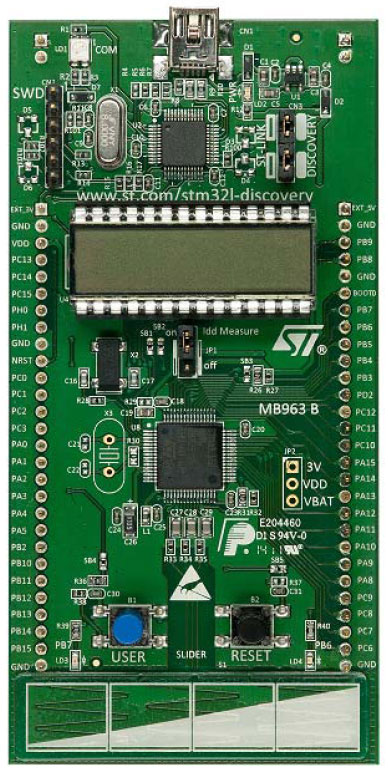
\includegraphics[scale=0.15]{img/stm32l_discovery.jpg}
				\end{figure}
			\end{frame}
			
			
		\subsection{Caractéristiques}
			\begin{frame}
				\frametitle{Caractéristiques}
				Microcontroleur
				\begin{itemize}
					\item Adresse 32 bits
					\item Mémoire
						\begin{itemize}
							\item Flash: 128 Ko
							\item RAM: 16 Ko
						\end{itemize}
					\item Others
						\begin{itemize}
							\item RTC (Real Time Clock)
							\item USART (Universal Asynchrone/Synchrone Receiver/Transmitter)
							\item I2C (Inter Integrated Circuit)
							\item SPI (Serial peripheral interface)
							\item ADC (Analog-Digital Convertor)
							\item DAC (Digital-Analog Convertor)
							\item Comparateurs
							\item ...
						\end{itemize}
				\end{itemize}
			\end{frame}
			
			\begin{frame}
				\frametitle{Caractéristiques}
				\begin{figure}
					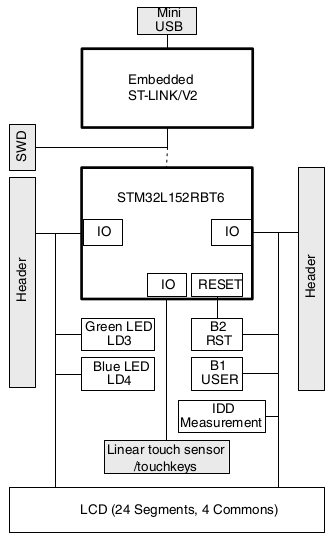
\includegraphics[scale=0.40]{img/shemaSTM32.png}
				\end{figure}
			\end{frame}
			
			
		\subsection{Utilisation}
			\begin{frame}
				\frametitle{Structure de la mémoire}
				\begin{figure}
					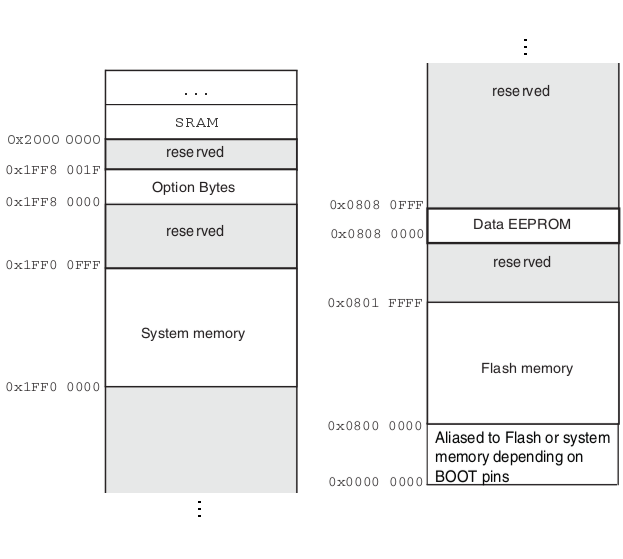
\includegraphics[scale=0.40]{img/memoire.png}
				\end{figure}
			\end{frame}
			
			\begin{frame}
				\frametitle{Structure d'un programme}
				Pour créer un executable ELF
				\begin{itemize}
					\item Code source
					\item Startup program
					\item Linker
				\end{itemize}
			\end{frame}
			
			\begin{frame}
				\frametitle{Structure d'un programme}
				\begin{figure}
					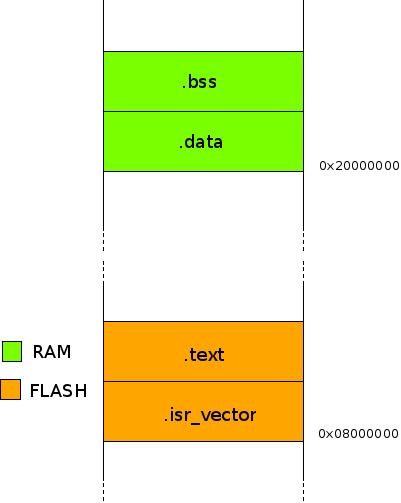
\includegraphics[scale=0.40]{img/ProgramMemory.jpeg}
				\end{figure}
			\end{frame}
			
			\begin{frame}
				\frametitle{Chargement sur la carte}
				\begin{alertblock}{ Prérequis }
					\begin{itemize}
						\item Suite de cross compilation (arm-none-eabi)
						\item Utilitaire texane-stlink
					\end{itemize}
				\end{alertblock}
				
				\begin{block}{ Procédure de chargement }
					\begin{itemize}
						\item Lancement de l'utilitaire texane-stlink
							\begin{itemize}
								\item \# ./st-util -p 4242
							\end{itemize}
						\item Chargement du programme avec GDB
							\begin{itemize}
								\item \# arm-none-eabi-gdb
								\item (gdb) target extended-remote :4242
								\item (gdb) load ./programme.elf
							\end{itemize}
					\end{itemize}
				\end{block}
			\end{frame}
	
	
	
	
	
	\section{Qemu}
		\subsection{Présentation}
			\begin{frame}
				\frametitle{Qemu}
				\begin{figure}
						
\includegraphics[scale=0.8]{img/qemu_logo.png}
					\end{figure}
				\begin{itemize}
					\item Emulation complète
						\begin{itemize}
							\item Intel
							\item ARM
							\item PowerPC
							\item Sparc
							\item ...
						\end{itemize}
					\item VMWare, Virtualbox, ...
				\end{itemize}
			\end{frame}
			
			
		\subsection{Utilisation}
			\begin{frame}
				\frametitle{Emulation d'un programme}
				\begin{block}{ Procédure de chargement }
					\begin{itemize}
						\item Compilation du programme utilisateur
						\item Lancement de Qemu avec le programme émulé
					\end{itemize}
				\end{block}
			\end{frame}
			
			
		\subsection{Structure}
			\begin{frame}
				\frametitle{Composant}
				\begin{figure}
					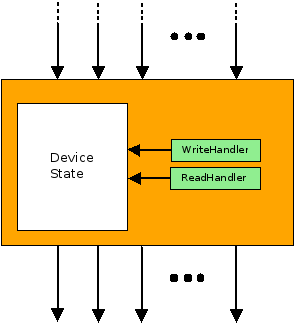
\includegraphics[scale=0.40]{img/shemaDevice.png}
				\end{figure}
				\begin{itemize}
					\item Etat du composant (Device State)
					\item Interfaces d'entrées (fils)
					\item Interfaces de sorties (fils)
					\item Gestion d'une zone mémoire déléguée
					\item Enregistré dans Qemu: Accessible pour les machines
				\end{itemize}
			\end{frame}
			
			\begin{frame}
				\frametitle{Machine}
				\begin{itemize}
					\item Qemu met à disposition des machines
						\begin{description}[flushleft]
							\item[Syborg]Platforme virtuelle Symbian
							\item[n800]Nokia N800
							\item[lm3s6965evb]Stellaris LM3S6965EVB
							\item[stm32l152rbt6]STM32L Discovery (Travail réalisé)
						\end{description}
					\item Assemblage de composants
					\item Communication avec des CharDev
				\end{itemize}
			\end{frame}
			
			\begin{frame}
				\frametitle{CharDev}
				\begin{itemize}
					\item Interface de communication
						\begin{itemize}
							\item Socket
							\item Clavier
							\item Port série
							\item ...
						\end{itemize}
					\item Bidirectionnelle
					\item Fonctionnement
						\begin{itemize}
							\item Initialisation au lancement de Qemu
							\item Connexion à l'initialisation de la machine
							\item Fonction d'envoi
							\item Handler de réception
						\end{itemize}
				\end{itemize}
			\end{frame}
			
			
			
	\section{Travail réalisé}
		\subsection{GPIO}
			\begin{frame}
				\frametitle{GPIO - Description}
				\begin{itemize}
					\item General Purpose Input/Output
					\item Entrée/Sortie pour usage général
					\item Paramètrable grâce à des registres de configuration
					\item Modes de fonctionnement
						\begin{itemize}
							\item Implémentés
								\begin{itemize}
									\item Output (Push/Pull)
									\item Input (Push/Pull)
								\end{itemize}
							\item Non implémentés
								\begin{itemize}
									\item Output (Open-drain)
									\item Input (Open-drain)
									\item Alternate function
								\end{itemize}
						\end{itemize}
				\end{itemize}
			\end{frame}
			
			\begin{frame}
				\frametitle{GPIO - Implémentation}
				\begin{itemize}
					\item Registres représentés par une structure
						\begin{figure}
							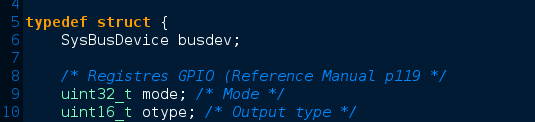
\includegraphics[scale=0.40]{img/structureGPIO.png}
						\end{figure}
					\item R/W en mémoire grâce aux fonctions handlers
						\begin{figure}
							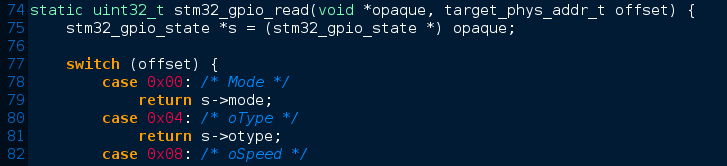
\includegraphics[scale=0.35]{img/handlerGPIO.png}
						\end{figure}
				\end{itemize}
			\end{frame}
		
		
		\subsection{LED}
			\begin{frame}
				\frametitle{LED}
				\begin{figure}
					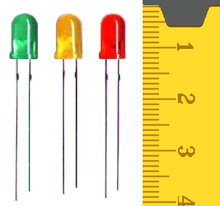
\includegraphics[scale=0.40]{img/led.png}
				\end{figure}
				\begin{itemize}
					\item Connexion à une sortie GPIO
					\item Envoi de l'état au CharDev quand la sortie GPIO change d'état
				\end{itemize}
			\end{frame}
		
		\subsection{Bouton}
			\begin{frame}
				\frametitle{Bouton}
				\begin{figure}
					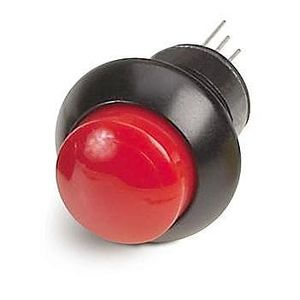
\includegraphics[scale=0.40]{img/bouton.jpg}
				\end{figure}
				\begin{itemize}
					\item Connexion à une entrée GPIO
					\item Envoi d'un signal au GPIO quand il reçoit un signal du chardev
				\end{itemize}
			\end{frame}
			
		\subsection{Machine}
			\begin{frame}
				\frametitle{Machine}
				\begin{figure}
					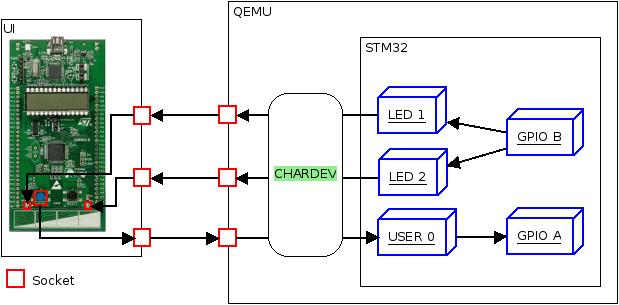
\includegraphics[scale=0.4]{img/machine.jpeg}
				\end{figure}
			\end{frame}
		
		
		\subsection{Différences avec la carte physique}
			\begin{frame}
				\frametitle{RCC}
				Realtime Clock Control
				\begin{block}{ Procédure d'écriture sur une pin GPIO }
					\begin{itemize}
						\item Parametrage via les registres
						\item Ecriture dans le registre "Output data"
						\item La valeur sera recopiée sur la pin au prochain tick de la RCC
					\end{itemize}
				\end{block}
				\begin{alertblock}{ Problème }
					Le module RCC n'a pas été implémenté dans Qemu
				\end{alertblock}
				\begin{exampleblock}{ Solution adoptée }
					Notre implémentation des GPIO recopie la valeur sur la pin sans attendre le tick de la RCC
				\end{exampleblock}
				
			\end{frame}
		
			\begin{frame}
				\frametitle{Zones d'adresse}
				\begin{block}{ Mapping d'adresses }
					\begin{itemize}
						\item Zone de boot pouvant être remappée en fonction des jumpers sur
							\begin{itemize}
								\item SRAM: Pour les tests
								\item Flash: Pour ecrire un programme persistant
							\end{itemize}
					\end{itemize}
				\end{block}
				\begin{alertblock}{ Problème }
					Ce remappage n'existe pas sur Qemu
				\end{alertblock}
				\begin{exampleblock}{ Solution adoptée }
					Création de 2 version de programme
					\begin{itemize}
						\item Qemu: le programme est "nativement" logé aux adresses de boot (0x0000 0000)
						\item Hardware: le programme est logé en flash (0x0800 0000) puis mappé materiellement sur les adresses de boot (0x0000 0000)
					\end{itemize}
				\end{exampleblock}
			\end{frame}
	
	
	\section{Démonstration}
		\subsection{GPIO Output}
			\begin{frame}
				\frametitle{GPIO Output}
				\begin{block}{ Déroulement }
					\begin{itemize}
						\item Initialisation des GPIO
							\begin{itemize}
								\item Le registre Mode
								\item Activation de la RCC pour le GPIO\_B (LED)
							\end{itemize}
						\item While(1)
							\begin{itemize}
								\item Switch\_LED\_ON()
									\begin{itemize}
										\item Ecrire dans le registre de sortie
									\end{itemize}
								\item Delay()
								\item Switch\_LED\_OFF()
									\begin{itemize}
										\item Ecrire dans le registre de sortie
									\end{itemize}
								\item Delay()
							\end{itemize}
					\end{itemize}
				\end{block}
			\end{frame}
			
			
			
		\subsection{GPIO Input + Attente active}
			\begin{frame}
				\frametitle{GPIO Input + Attente active}
				\begin{alertblock}{Limite}
					Nous n'avons pas implémenté les interruptions processeur pour pouvoir utiliser des handlers d'interruption.
					Ce programme réalise donc une attente active
				\end{alertblock}
				\begin{block}{ Déroulement }
					\begin{itemize}
						\item Initialisation
							\begin{itemize}
								\item GPIO\_B en sortie, GPIO\_A (Bouton) en entrée
								\item Activation de la RCC pour les GPIO
							\end{itemize}
						\item While(1)
							\begin{itemize}
								\item Si l'état a changé
									\begin{itemize}
										\item Switch\_LED()
									\end{itemize}
							\end{itemize}
					\end{itemize}
				\end{block}
			\end{frame}
	
	

	
	
	\section{Conclusion}
		\subsection{Prochaines évolutions}
			\begin{frame}
				\frametitle{Prochaines évolutions}
				\begin{itemize}
					\item Gestion des interruptions materielles
					\item Implémentation des protocoles (Alternate function)
					\item Implémentation des composants (Ecran, ADC, ...)
					\item Implémentation du composant RCC et des Timers
				\end{itemize}
			\end{frame}
		
		\subsection{Rétrospective}
			\begin{frame}
				\frametitle{Rétrospective}
				\begin{alertblock}{ Points négatifs }
					\begin{itemize}
						\item Temps pour appréhender le système Qemu
						\item Temps pour appréhender le hardware
					\end{itemize}
				\end{alertblock}
				\begin{exampleblock}{ Points positifs }
					\begin{itemize}
						\item Utilisation des CharDev
						\item Compréhension des mécanisme de Qemu
						\item Documentation du Wiki Qemu
					\end{itemize}
				\end{exampleblock}
			\end{frame}

		\subsection{Questions}
			\begin{frame}
				\frametitle{Questions}
				\begin{figure}
					
\includegraphics[scale=0.4]{img/question.jpg}
				\end{figure}
			\end{frame}
			
			
\end{document}

